% Created 2020-04-23 Thu 16:29
% Intended LaTeX compiler: pdflatex
\documentclass[11pt]{article}
\usepackage[utf8]{inputenc}
\usepackage[T1]{fontenc}
\usepackage{graphicx}
\usepackage{grffile}
\usepackage{longtable}
\usepackage{wrapfig}
\usepackage{rotating}
\usepackage[normalem]{ulem}
\usepackage{amsmath}
\usepackage{textcomp}
\usepackage{amssymb}
\usepackage{capt-of}
\usepackage{hyperref}
\usepackage{geometry}
\usepackage{charter}
\usepackage{booktabs}
\usepackage{float}
\author{fbi}
\date{\today}
\title{}
\hypersetup{
 pdfauthor={fbi},
 pdftitle={},
 pdfkeywords={},
 pdfsubject={},
 pdfcreator={Emacs 26.3 (Org mode 9.1.9)}, 
 pdflang={English}}
\begin{document}

\begin{titlepage}
   \begin{center}
       \vspace*{1cm}


        {\textsc{\large ENEL 300: Electrical Engineering Design}}

        \vspace{0.5cm}

        \textsc{\textbf{\huge  Final Technical Report: iDrops}}
 
        \vspace{0.3cm}

        {\textsc{\large For Learning community 7 Group 1}}
 
       \vspace{1.5cm}
 
       \begin{tabular}{l r}
         \toprule
          \textbf{Course Instructor} & Dr. Laleh Behjat \\
         \bottomrule
       \end{tabular}
 
       \vfill
 
       \begin{tabular}{l}
       \textbf{Group Members} \\
       \midrule
       Tomin Mattam \\
       Tahseen Intesar \\
       Eduard Pjetracaj \\
       Jordan Lonneberg \\
       \bottomrule
       \end{tabular}
 
       \vspace{0.8cm}
 

   \end{center}
\end{titlepage}

\section{Introduction}
\label{sec:org0a35038}
Our product is a simple drum machine. A drum machine is a musical
instrument that enables people to make loops of musical samples which
serve as the beats for songs. With our drum machine, a user can select
between a number of built-in samples - for example, a kick drum,
snare, Hi-hat, tom -- or load custom samples of their choosing.  They
can then select when each instrument will be played within the drum
loop forming a \emph{pattern} which the drum machine plays back as a loop.
From here, the user can apply a number of effects to each sample to
tweak the sound of the beat to their liking. Once the user is
satisfied with the results of the sound, they can export the drum loop
to a ".wav" file to be played back over vocals or other instruments.

One of the major issues with current market offerings in this segment
are the steep learning curves and high costs (often upwards of 400
dollars). This makes the idea of getting started learning music
production with these drum machines daunting and opaque, dissuading
many from even trying to pursue this hobby. One current solution to
the problem issue of cost has been the proliferation of digital audio
workstations (DAWs), which can provide a full music production setup
for only a few hundered dollars, however they have a number of hidden
costs. First is their enormous complexity, these DAWs are design to
suit any number of music production setups and aim to allow producers
to mix full songs inside of a single application. Although this makes
them powerful for users who are experienced in these software
solutions, it results in a convoluted and inconsistent application
that takes a career to master and learn how to use
correctly. Secondly, using just a mouse and keyboard with these
applications to make music is \emph{hard}, and those who use them regularly
use external MIDI devices that allow them to play virtual instruments
in the same way they would play a piano, but again these external MIDI
devices cost money - quite a bit for a good piece of kit - and add to
the cost of anyone interested in using software to get acquainted with
music production. For these reason, we see that the current market for
music production hardware and software fails to make it easy for
beginner producers and musicians to get started production, and our
product aims to solve this issue by being cheap and easy to use.

Our drum machine aims to be fairly simple having the ability to switch
between 8, 12 and 16 beats per loop, and sticking to a restricted
sub-set of only the most important effects. By keeping our product
design and function simple - as compared to many existing products -
we aim to streamline our products use and keep the cost of production
and design low which will help target our ideal user persona.

\section{Persona and Product}
\label{sec:org2c3e213}
\subsection{Persona}
\label{sec:orgdf33ceb}

Our drum machine focuses on anyone around the world who wants to get
into music production but does not have a lot of money to spend on a
drum machine. As we have outlined above (and in our market research
Section \ref{org44573e9}), current product offerings do not target beginners
to the hobby of music production. Generally, these offerings cost too
much for a young person to afford and have a steep enough learning
curve that many are dissuaded from buying them. The key points of
our user persona are as follows:

\begin{itemize}
\item Young adults (target age of 13 to 19).
\item Thrifty, our target users are budget conscious and are always looking for the best deal around.
\item Wants to get started in music production but has little prior experience. May already have some experience, but is at a novice level.
\end{itemize}


When we interviewed a group member’s relative, who expressed her
interest in wanting to become a musician; however, she lacked the
funds and expertise to start when she was younger. When we approached
her with the idea of a drum machine, she found it interesting how
simple the concept was, and that she wished that a product such as the
iDrop was available to her when she wanted to get into music.

Below are a few samples of user-stories we found on the internet. Generally,
we found that many people were frustrated by the opaque interfaces of many
DAWs. \emph{Note: The quotes below are clickable links to the source comments.}

\begin{itemize}
\item \href{https://www.amazon.ca/gp/customer-reviews/R1OFNI0GNZ2VC?ref=pf\_vv\_at\_pdctrvw\_srp}{ Complicated to use. Limited options. Requires non standard power supply, plug on standard wall wart doesn't fit.} - Amazon review for Korg KR mini Rhythm Machine.
\item \href{https://www.quora.com/Is-FL-Studio-easy-to-learn}{No it isn't \ldots{} FL Studio is a highly complex and disorganized piece of software} - Answer to question about if FL studio (a DAW) is easy to use.
\item \href{https://www.kvraudio.com/forum/viewtopic.php?f=7\&t=360703\&sid=2d239239fdd437172d4208545e3d608b}{"I really like FL, and it's one of the most capable I own (and I own most). However, I rarely use it because it differs so much from standard Windows behaviour - the right-click especially, and so I always end up doing the wrong thing (I'm always right-clicking clips to get properties, and then finding I'm un-painting them, etc.)." }
\item \href{https://sound.stackexchange.com/questions/25161/why-is-learning-how-to-use-daws-appear-more-difficult-than-video-editing-program}{ The only thing I can think of with music production software is the fact you're dealing with multiple concepts. When using music production software it may help to separate each area into it's constituent components and study them that way.} - response to stackexchange question asking why DAWs are hard to use.
\end{itemize}

For our user persona, our user is a teenager named Gent
Mattberg from Atlanta,Georgia who always wanted to be a young famous
musician but still anxious whether he would also be undiscovered. The
data shows that almost 90.7\% of all artists are undiscovered, 6.8\%
are developing, 1.4\% are mid-sized, 0.9\% are mainstream, and only 0.2\%
are considered megastars
\footnote{https://blog.nextbigsound.com/next-big-sounds-state-of-the-industry-2013-e2edd4d0f897}. So
there is a very long road to go to be a mainstream artist and make a
living. Our aim is to allow budding musicians to achieve their dream
because by giving them access to music production at a lower cost than
ever before.


\begin{sidewaysfigure}
\centering
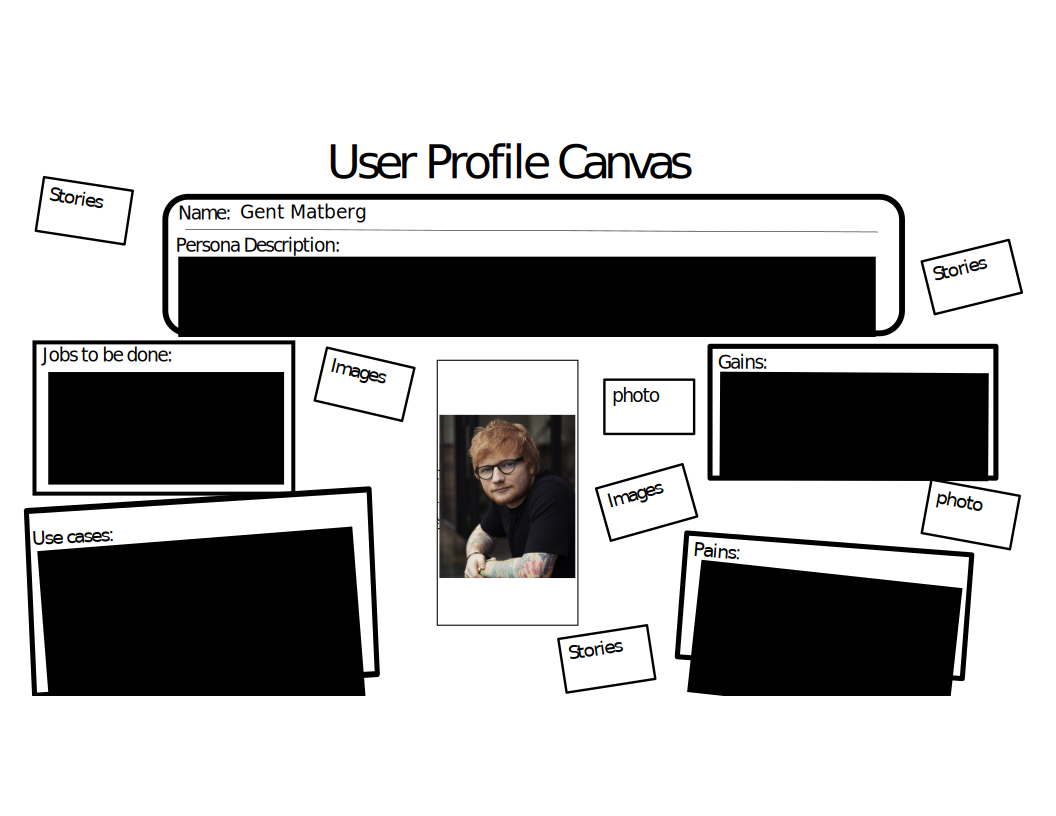
\includegraphics[width=15cm]{./profile_canvas.png}
\caption{\label{fig:orgec983ae}
A filled out empathy map for our product.}
\end{sidewaysfigure}

\newpage


\begin{figure}[H]
\centering

\includegraphics[width=10cm]{./empathy_map.png}
\caption{\label{fig:org2e4a1e3}
A filled out empathy map for our product.}
\end{figure}

\subsection{Product}
\label{sec:org1f0f98b}

   As we have discussed before, we aim to target people who have an
interest in music production but have little prior experience. The 
current predicament 

So at the same time these people are trying to grasp fundamental
concepts of music production while also trying to make sense of
confusing software solutions. These users could go out and purchase
some dedicated hardware however existing solutions however many of
these are prohibitively expensive (see Section \ref{org44573e9} for more
analysis of existing solutions). Our goal is to fix this by providing
a few key features:

\begin{itemize}
\item Low cost (around \$85).
\begin{itemize}
\item Our users are value oriented, so we need to distinguish our product
\end{itemize}
\end{itemize}
by keeping prices low.
\begin{itemize}
\item Small and compact.
\begin{itemize}
\item This helps to keep costs low, and we think that buying our product
should not be a huge investment in space either, so it should not
be hard to stow away.
\end{itemize}
\item Sample based playback.
\begin{itemize}
\item Allows users to drag and drop clips of drum from their computer
onto an SD card so they can play back any sound they want.
\item This makes the product of versatile, as it can playback a theoretically
infinitely different number of drum-kit setups.
\end{itemize}
\item MIDI support.
\begin{itemize}
\item MIDI is a standardized way for musical instruments to communicate with each other. By
adding MIDI support to our product, users can hook this up to
any existing instruments they have, and it allows the product to
still be useful as our users begin using more powerful tools
like DAWs.
\end{itemize}
\end{itemize}

First, it is important to breakdown why we choose these as important
factors instead of some other set of criteria. We see low cost as an
important criteria as we are marketing to young adults who generally
do not have large sums of disposable income. So to our target persona,
any price over 100 dollars rapidly becomes a large investment. Given that
we want to capture anybody with an interest in music production - even
those with a minor interest - a lower cost device is much more appealing
as it represents less of an investment.

Sample based playback also has the advantage of allowing the user to
use effects not directly supported by our device. Due to the low-cost
nature of our device, it will have a limited sub-set of effects that
can be applied to samples. Some users may not find these effects
enough to make the exact sounds that they want but due to use using a
sample-based approach, the user can just open it in a simple audio
editor like the free editor \href{https://www.audacityteam.org/}{audacity}. Unlike DAWs, these applications
are generally easy to use, and come with many built-in effects. Once
the user is happy with the sound that they get with the software, they
can drag-and-drop it onto and SD card to be played back with the drum
machine. So by using our sample-based approach - as opposed to a
\emph{wavetable synthesis} approach, we are able to leverage easy to use
existing computer software to make our device more flexible and
powerful.

One of our goals was also to implement basic MIDI support. As
mentioned in the introduction, professional and hobbyist producers
often use an external keyboard or sequencer to make the usage of DAWs
easier.  Although our product is aimed at beginners and this is a more
"advanced" feature, one issue with trying to sell an extremely
bare-bones system is getting users to justify the cost of our
product. Although our product is much cheaper than existing solutions,
many potential users may feel that they would rapidly outgrow the
product if the feature set was too limited. This would result in many
users who could genuinely benefit from the product avoiding buying it
because they see it as a poor investment which will have limited
long-term utility. By adding MIDI support, we are allowing our product
to grow with the user as they become more advanced. As users gain more
experience in music production they will inevitably gravitate to more
sophisticated methods like DAWs and the MIDI support would allow these
users to continue using our product as a sequencer even though they
have outgrown the built-in effects. In a sense, MIDI support allows
our product to be a supplement to DAWs, and acts as a stepping stone
to more advanced and challenging methods of music production improving
the value to the customer as it extends our products utility.


Based on our market analysis, we found that our device is high-impact
as it fills a niche within the musical instrument market that has yet
to be targeted. Based on our product value canvas (Figure \ref{fig:org5c053a1}) we
found that our product has a unique value proposition as it offers a
powerful sample-based approach to drum machines at a low-cost --
something that current market offerings do not. Figure \ref{fig:orgcf5c438} show
an earlier impact versus feasibility analysis done during the
entrepreneurship workshops. From this we also found that our device is
high impact, however at the time there were some questions about our
market size and profitability.  These concerns have been addressed and
can be found inside our investor pitch.

\newpage

\begin{sidewaysfigure}
\centering
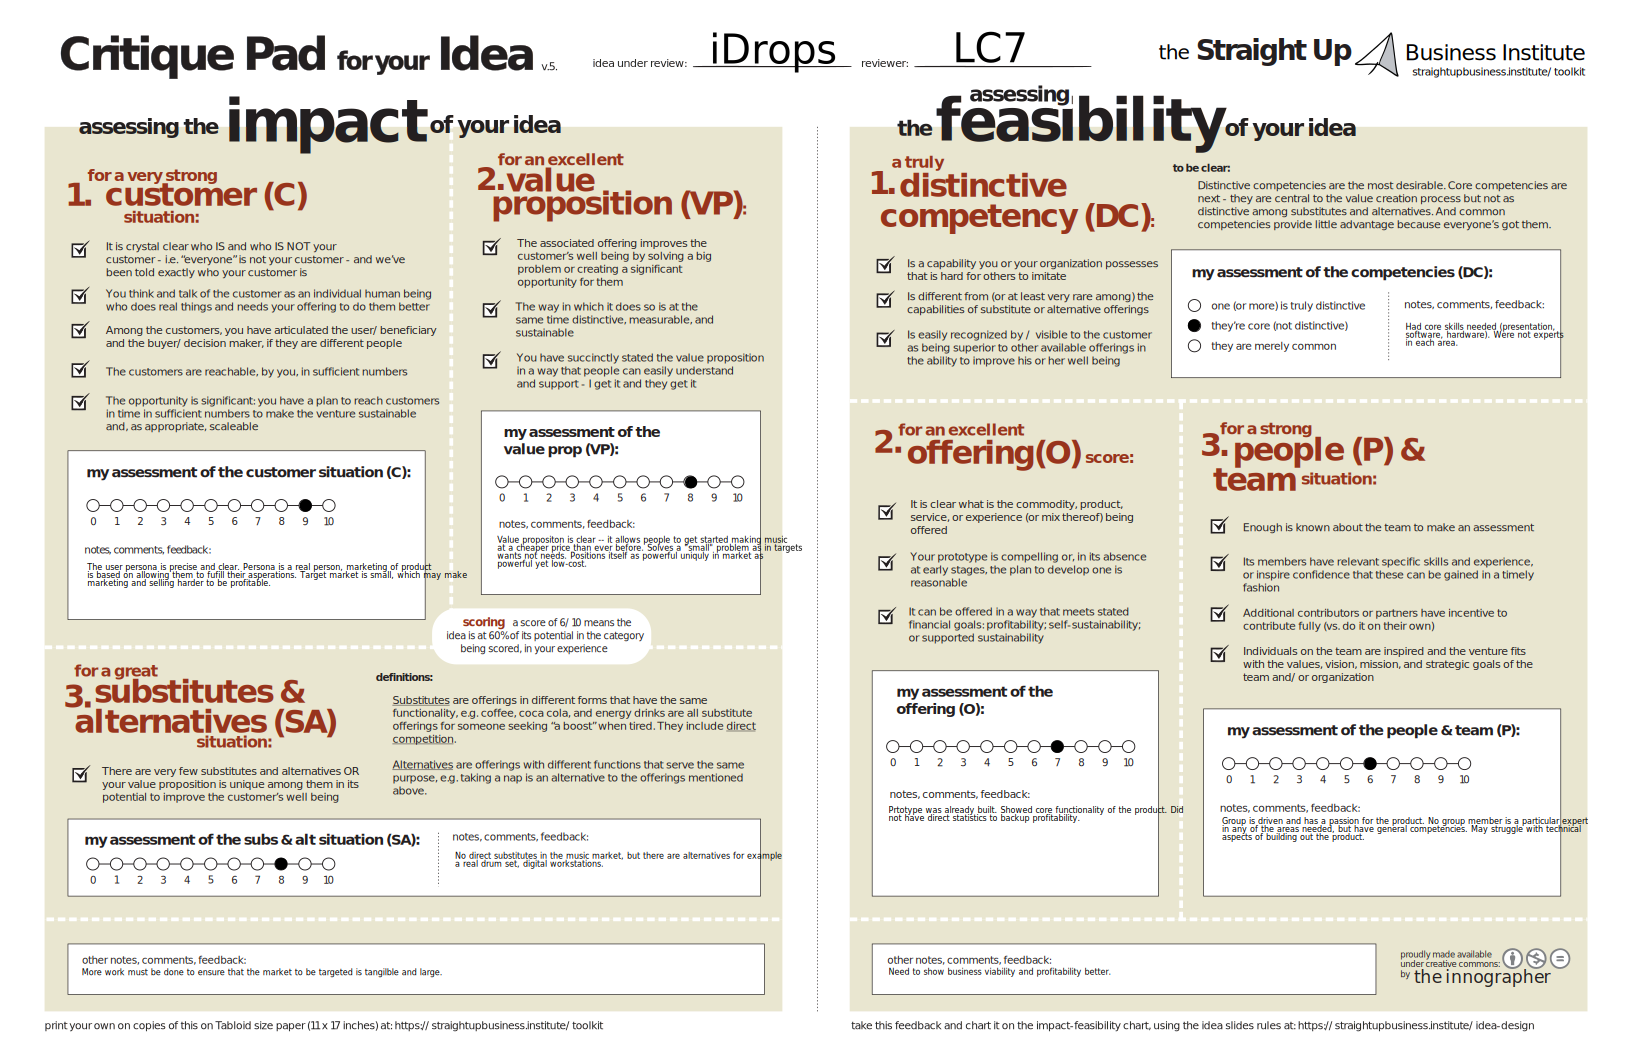
\includegraphics[width=22cm]{./impact.png}
\caption{\label{fig:orgcf5c438}
The impact versus feasibility chart we performed during the entrepreneurship workshops. Not indicative of current project state, we have addressed concerned over marketability as dicussed in our investors pitch.}
\end{sidewaysfigure}

\newpage

\begin{figure}[htbp]
\centering
\includegraphics[width=15cm]{./pvc.png}
\caption{\label{fig:org5c053a1}
Value propositon canvas for our product.}
\end{figure}

\subsubsection{Market research}
\label{sec:org5e132ec}
\label{org44573e9}

    Because we are targeting a space with existing products, one of
our first tasks was to assess existing market offers. We identified
two existing products that are in a similar price range (sub \$400
range) and could have a similar value proposition.

 The first product is the \href{https://teenage.engineering/products/po-32}{teenage engineering PO-32} which comes in at
a base price of about 120 dollars. In terms of cost this is the
offering that is the closest to matching our pricing scheme. There are
a few issues with this product. The first is that it is a \emph{drum
synth}, meaning that it uses waveshaping and wavetables to generate
sounds that emulate the instruments of a drum-kit. This is in contrast
to our machine which directly uses audio clips of real-life drum kits
to produce drum sounds. Although in some cases the sound from the
synthesis method of sound production is desirable, it is more limited
in the range of sounds it can produce making this a net disadvantage
as it limits the power of the drum machine for no real reason. A
second issue is its appearance and user-experience. The PO-32 uses the
same tiny push buttons that people often like to use on their DIY
project which are fine for prototyping, but they are hard to push
quickly and are fragile. The PO-32 is also shipped as a bare pcb
without any case making the device fragile and contributes to a
overall toy-like feel. You can buy a silicone case for the PO-32 to
fix some of these issues, but that brings to total price of the device
up to \$160 and still is not as good as a proper hard plastic
case. Finally, although this device has gotten very good reviews, most
of the praise is centered around its additional software plug-in
called "microtonic", which costs and additional 140 dollars and
requires the user to already own a DAW to get good functionality out
of. For these reasons, we see this device as not effectively catering
to the beginners market because in order to get good functionality you
need to own software which few beginners will have, and it still has
the issue of beginners having to learn a DAW in order to get started
-- which is something we want to avoid to streamline getting into
music production.

The second product is the \href{https://www.korg.com/caen/products/dj/volca\_beats/}{Korg volca beats} which comes in at 210 dollars.
Again, the issue with this drum machine is that it is an \emph{analogue synth} style
machine not based on using samples making the range of sounds it can produce
limited in comparison.

\section{Technical Description}
\label{sec:org473b58b}
\subsection{Pre-COVID technical description}
\label{sec:orgfca4953}
\begin{figure}[H]
\centering
\includegraphics[width=10cm]{./side profile.png}
\caption{\label{fig:orgc511e8e}
A CAD drawing of our physical product that could not be built due to COVID-19.}
\end{figure}

Figure \ref{fig:org4582cc7} shows a block diagram of how our product is
contracted on a high level. Originally, we planned to power our device
using a 5 volt adapter from a wall socket - preferably USB due to its
ubiquity. The operation of our device would be as follows. First the
device would load the samples to be played back off of the SD card
into memory. It would then monitor for buttons presses which would
turn on and off each instrument at a specific \emph{tick} as the drum
machine looped around. The buttons on the left of the device would
allow the user to select which instrument would be currently
selected. The knobs would allow users to adjust a number of the
samples parameters and shape the waveform to a desired sound. These
knobs would be a simple potentiometer circuit seen in figure
\ref{fig:org1fb9636}. Figure \ref{fig:org66f1cec} shows a simple switch circuit that would
allow us to hook up multiple switches to each pin. We had planned to
replace some of these switches with capacitive touch buttons as per
instructor recommendations however we did not get to drawing this
circuit by the time classes were canceled. Figures \ref{fig:org730aa01} and
\ref{fig:orgeb2729d} show LED driver circuits we had designed. Eventually we
settled on using the circuit in Figure \ref{fig:orgeb2729d} as it reduced the
number of PIC16 pins used to drive the LEDs, would make board layout
much easier, and would give us experience using I2C. We also had
planned a few other features such as a hybrid-approach to sound
synthesis which would use the SD card samples in conjunction with
wavetable synthesis. Much of our original projects difficulty stemmed
from the software side of the design, in particular it required very
tight timing requirements given the relatively complex maths we needed
to do during our waveshaping stages of the program and the lack of
a DMA controller on the PIC. Unfortunately none of this was written by
the time classes were canceled and thus cannot be demonstrated.

\begin{figure}[htbp]
\centering
\includegraphics[width=8cm]{./block_diagram.png}
\caption{\label{fig:org4582cc7}
Block diagram of our product.}
\end{figure}

\begin{figure}[htbp]
\centering
\includegraphics[width=4cm]{./pot.png}
\caption{\label{fig:org1fb9636}
Very simple circuit used to get potentometer inputs for knobs.}
\end{figure}

\begin{figure}[htbp]
\centering
\includegraphics[width=7cm]{./LED_matrix.png}
\caption{\label{fig:org730aa01}
An earlier LED driver circuit we were working on. We decided that this circuit was not suitable for a number of reasons. First, it requires 8 pins to drive meaning we are sacrificing an entire port just to using LEDs. Second, our led arrangment would not actually be a square matrix, making the layout of this circuit for our product would be impossible to do cleanly.}
\end{figure}

\begin{figure}[htbp]
\centering
\includegraphics[width=10cm]{./led_driver_newpng.png}
\caption{\label{fig:orgeb2729d}
A circuit shematic for an alternate LED driver. This design was considered favourable for two reasons. First it would give us experience with using I2C unlike the other one. Additionally it does not require us to sacrifice an entire port to just driving LEDs. Here Rext was found to be 750 ohms based on page 9 of the TLC9116 datasheet.}
\end{figure}

\begin{figure}[htbp]
\centering
\includegraphics[width=4cm]{./switch_circuit.png}
\caption{\label{fig:org66f1cec}
A switch multiplexer circuit which allows mutiple switches to be mapped to one alalog input pin. Our device would require 3 of these circuits.}
\end{figure}

\newpage 
\subsection{Post-COVID technical description}
\label{sec:org6791b4e}
   For the post-COVID prototype, we have decided to move forward using
software to emulate some of the key aspects of our design. To do so,
we have created a GUI software the provides some of the basic
principles of our product idea. Our original prototype written in C
had the core feature set of our product, but it lacked a number of key
features that our product needs in order to be a viable product.  For
the core features that we wanted to add to our implementation we came
up with the following:

\begin{itemize}
\item Support for some basic audio effects (e.g, echo, bitcrushing, etc).
\item Make the beats per minute adjustable.
\item Allow loading custom samples.
\item Improve user experience by creating a GUI.
\item Keep the product as faithful to the original as possible.
\begin{itemize}
\item This means that the final product should still be as small and resource construed as the originally planned PIC16 code because this would make porting the software over easier.
\end{itemize}
\item Support for exporting drum loops as audio files.
\end{itemize}


For reference of our starting point Figure \ref{fig:org2bc6f83} shows an example of
the early prototype in action. This early prototype lacked a number of
current features, notably the loaded ".wav" sample files were
compile-time constants, the beats per minute (BPM) was a compile-time
constant, and there were no audio effects available.

\begin{figure}[htbp]
\centering
\includegraphics[width=5cm]{./TUI.png}
\caption{\label{fig:org2bc6f83}
A screenshot of the early terminal prototype. Users could use the "qwertyuiop[]" keys to select when a particular instruments would play, use the number keys to select the the current instrument, and use the m, +, and - keys for muting, making louder, or making qiuter the current instrument.}
\end{figure}

The basic operation of our GUI is as follows. By default, the
left-hand side of the application has a "sequencer" tab in which the
user can click on buttons to enable or disable the instrument on a
particular beat. This is where a user can specify the progression of a
beat and when certain samples are played in the loop. On the right
hand side by default is a tab which holds the users options. The
global options are the beats per minute and global
volume. Additionally, under the options the user can specify effects
for each musical instrument, for example muting that instrument in the
loop, clearing the loop pattern for a specific instrument, changing
the gain for a single instrument, or applying an echo effect. This is
seen clearly in Figure \ref{fig:org1c2ae93}. To see a video of our product
being used, please see the included demo footage.

\begin{figure}[htbp]
\centering
\includegraphics[width=15cm]{./GUI_1.png}
\caption{\label{fig:org1c2ae93}
A screenshot of a newer GUI prototype showing basic operation. The large squares on the left are the buttons which users can specify what pattern they want each instrument to play on during the drum loop. The dots below the buttons indicate which tick is currently being played. On the right are some options for global and per-instrument effects. The option panel also contains buttons to export the drum loop to a ".wav" file, and to change the currently selected drum-set.}
\end{figure}

Our program also has the ability to load users custom samples through
a simple config system. The program is designed to search for any
".idc" files (the file extension stands for idrops configuration) and
open it. The configuration files are simple plain text files that are
formatted as \texttt{key : "value"} where the key is the name of the
instrument, and the value is the file path of the audio file for that
instrument. For example, the built-in tr-909 configuration file is seen in
Figure \ref{fig:orgbb8b843}.

\begin{figure}[H]
\centering
\includegraphics[width=7cm]{./config.png}
\caption{\label{fig:orgbb8b843}
The contents of "tr909.idc" which is in the provided source code.}
\end{figure}

The program searches for all ".idc" files and parses them at start-up,
allowing the user to select from many different drum sets. The user
can have as many ".idc" files as they want, allowing the user to
switch which drum samples they are using on the fly. This is seen in
Figure \ref{fig:org00ba6c3}, which shows a drop-down menu with a few built-in
drum sets.

\begin{figure}[htbp]
\centering
\includegraphics[width=10cm]{./drum_sets.png}
\caption{\label{fig:org00ba6c3}
A screenshot showing the drop-down menu for selecting drum sets. Users can write their own ".idc" files to create their own custom drum-sets from easy to find ".wav" files on the internet. The parser for the ".idc" files was written by us - not using a library.}
\end{figure}

The software would be useless without the ability to export the drum
loops, so that has also been built into the software. With our software,
the user can click the "export loop to file" button which brings up a dialog
box allowing the user to give a name to the saved file. Figure \ref{fig:org988a589} shows
a screenshot of this dialog box being used.

\begin{figure}[htbp]
\centering
\includegraphics[width=10cm]{./file_export.png}
\caption{\label{fig:org988a589}
A screenshot of the export to file dialog box. The user can type a filename into the box and click the save button to export their drum loop.}
\end{figure}

Additionally, a side-effect of the GUI toolkit we are using is support
for custom color-schemes which although not strictly a technical
requirement we aim to fulfill some of these alternate color schemes
provide higher contrast and thus better accessibility. This is seen
in Figure \ref{fig:orga7cc4b1}.


\begin{figure}[htbp]
\centering
\includegraphics[width=15cm]{./GUI_2.png}
\caption{\label{fig:orga7cc4b1}
A screenshot of a newer GUI prototype showing support for themes.}
\end{figure}

Currently, our software is written in plain C99 and based on
\href{http://www.portaudio.com/}{portaudio} for the underlying API for playing sound, \href{http://www.mega-nerd.com/libsndfile/}{libsndfile} for
opening users ".wav" files for custom samples, and \href{https://github.com/Immediate-Mode-UI/Nuklear}{nuklear} for the GUI
framework. If you would like to see the source for the program or run it
yourself, please see the accompanying directory called "idrops\(_{\text{software}}\)".

\section{Teamwork and agile development}
\label{sec:org9ec371a}

We all shared the same vision from the very first day we were assigned
to work as a team, the vision of innovating an engineering
marvel. Teamwork is often a dream task, which is expressed not only in
the success of a team but also in individual development. We all knew
that we were from different scenarios in life and hence we were very
successful in dividing each tasks into tiny jobs among us depending on
our abilities and availabilities.In addition to that, our daily
stand-up meetings gave us the understanding on what we have done so
far and what was left to accomplish. In addition, using agile scrum
project management, we had an good understanding of how our product
was going to be, which gave us the opportunity to build our initial
prototype at the very beginning and allowed us to add more and more
detail through demand and regular testing.

For organizing our work we made extensive use of Trello and online
group-chats. For our usage of Trello we split each sprint into it's
own board for easier organization. On each of these Trello boards we
would organize columns for our "swim-lanes" of what tasks we needed to
do for that sprint how long each one was estimated to take and which
person was to do what with checkboxes that we could tick when we
finished a task. Generally we tried to keep our expectations for most
sprints reasonable by limiting the amount of work done by each person
to around 5 hours, which helped give a reasonable timeline for the
work to be completed. We also generally tried to keep the number of
hours done by each person even, however there were a few times during
our post COVID project development that some group members were busy
with family stuff, so during these weeks we felt it was more fair to
give them less hours and let the rest of us pickup to rest. For
meetings we tried to have some form of communication everyday --
usually through text-based chats. For these chats we would say how far
completed each of our tasks are, and give a time estimate of what was
left. We also had regular group video calls every Monday, Wednesday,
and often Friday on zoom after the transition to online-only
learning. During these video calls we would discuss new ideas that we
could add for the next sprint and would update our logs about which
tasks had been completed.

In terms of the benefits we saw from teamwork and agile development,
the scrum-based method of project management was helpful in that it
kept in our minds the idea of a persona. Every time we would modify or
analyze our product offering, it was through the scope of trying to
make what best fit the needs of our persona. Weekly sprints also made
sure that we had reasonable expectations of what could be performed
and ensured that we actually completed the tasks assigned. The scrum
method of development also helped with our post COVID-19 product
offering. We were able to quickly assess if our product could still be
built under the circumstances and found that creating a software
simulation of our product would be an excellent method of showing our
core product ideas even though we did not have the means to build a
physical prototype.

In particular the concept of a persona was helpful in establishing our
vision and what products we may be competing with. By developing the
persona of new and cash-strapped producers, we were pushed into do
research into existing products and found that there are no offerings
like ours.

\section{User manual and instructions}
\label{sec:org50b9233}
For the user manual, please see the accompanying file called
"user$\backslash$\(_{\text{manual.pdf}}\)".
\section{Intellectual property}
\label{sec:org32775c9}
\emph{Note: the "link" texts in this section will link directly to the searches that we performed, so please click on the if you want verification of our results or methodology.}

\subsection{Trademarks}
\label{sec:org8f81b9d}
Using the WIPO trademark search (\href{https://www3.wipo.int/branddb/en/}{link}), we found a total of 39 trademarks
that involved either the works "iDrop" or "iDrops".  Of these results
zero were pending or active inside of Canada. By region there were 13
US trademarks, 7 Mexican trademarks, and the rest mostly being
European. Our product fits into the NICE classifications 15 (musical devices),
28 (toys) (\href{https://www.wipo.int/classifications/nice/nclpub/en/fr/}{link}), which these two WIPO search results had zero (0)
trademakrs registered inside the same classes.

Additionally, based on a direct US trademark search (\href{http://tmsearch.uspto.gov/bin/showfield?f=toc\&state=4808\%3Ai92r0g.1.1\&p\_search=searchss\&p\_L=50\&BackReference=\&p\_plural=yes\&p\_s\_PARA1=\&p\_tagrepl\%7E\%3A=PARA1\%24LD\&expr=PARA1+AND+PARA2\&p\_s\_PARA2=idrops\&p\_tagrepl\%7E\%3A=PARA2\%24COMB\&p\_op\_ALL=AND\&a\_default=search\&a\_search=Submit+Query\&a\_search=Submit+Query}{link}) we found that
of currently live trademarks three (3) were related to online shipping, one (1)
was related to literal eye drops, and one (1) was related to purchasing online
pharmaceuticals.

Given that multiple search methods found that no other patents with
the similar names or logotype that are in similar classes to ours, we
can safely say that our product name does not violate any trademarks
with respect to the "iDrops" branding. This is also based on a discussion
we had with Jim Wilson in which he said that our product could have the
same trademarked name as an existing company or product as long as they
are not competing for the same markets as we are.

\subsection{Patents}
\label{sec:orgdce8a6d}
A patent search on Google patents (\href{https://patents.google.com/?q=\%22drum+machine\%22,\%22drum-machine\%22,\%22drummachine\%22}{link}) we found that the patents overwhelmingly 
related to washing machines and not musical instruments. Additionally, looking
at the patent assignees we found that zero of the companies with patents matching
these keywords are involved in musical instruments production or marketing.

It is important to note that words "drum machine" or any combination
thereof are generic both in the name and concept given that many
different manufactures have built these interments without approval
from each other.

From this, we can safely say that the term and concept of a "drum machine" that
we use is not patent encumbered. 
\end{document}